\documentclass[a4paper]{article}[25.12.2015]
  \usepackage[english]{babel}
  \usepackage[utf8]{inputenc}
  \usepackage[T1]{fontenc}
  \usepackage[text={17cm, 24cm}, left=2cm, top=3cm]{geometry}

%  \usepackage{amsmath}
%  \usepackage{amsfonts}
%  \usepackage{hyperref}
  \usepackage{graphicx}
  \usepackage{syntax}
  \usepackage{listings}
  \usepackage{float}

\begin{document}
%%%%
%%%%%
%file: title.tex
%date: 25.12.2015
%author: Jan Wrona
%email: <xwrona00@stud.fit.vutbr.cz>
%project: VYPe15 programming language compiler implementation, VYPe
%%%%%
\begin{titlepage}
\begin{center}
\textsc{{\LARGE Brno University of Technology}\\
\smallskip
{\Large Faculty of Information Technology}}\\
\vspace{\stretch{0.382}}
{\LARGE Compiler Construction}\\
\medskip
{\Huge VYPe15 programming language compiler implementation}\\
\vspace{\stretch{0.618}}
\end{center}
{\Large Jan Wrona, xwrona00:50\,\%}\\
{\Large Kateřina Žmolíková, xzmoli02:50\,\%}\\
{\Large Extensions: none \hfill \today}
\end{titlepage}
%%%%

%%%%
\section{Front end}
%%%%
Compiler front end reads the source code in source language, verifies its syntax, performs several semantic checks and generates an intermediate representation in the form of three-address code.
It is implemented in the C language with the help of tools \texttt{flex} and \texttt{bison}.
\subsection*{Lexical analysis}
Lexical analyzer source code is located in the file \texttt{scanner.l}.
It is intended to be used as an input file for the \texttt{flex}, which is a tool for generating programs that perform pattern-matching on text.
Definitions section contains declarations of two simple "name" definitions for escape characters and for other characters, to simplify the scanner specification.
Another declaration is for multi-line comments.
Rules section contains rules for single and multi-line comments, keywords, reserved words, identifiers, literals, operators, other needed characters and finally whitespaces.
User code section contains mainly functions for de-escaping characters and whole strings.
\texttt{flex} tool will generate C source file \texttt{scanner.c}, which is later compiled and linked with the rest of the compiler.

\subsection*{Syntax and semantic analysis}
Syntactic analyzer together with semantic actions is located in the \texttt{parser.y} file.
It is a source code for the \texttt{bison} tool, which is a parser generator.
Prologue section contains all the necessary C includes, definitions of the data structures, definitions of the global variables and function prototypes.
Declarations sections contains the names of the terminal and nonterminal symbols, describes operator associativity and precedence.
In the form of union, data types of semantic values are declared as follows:
\begin{lstlisting}[language=C]
union {
  char *identifier;
  int int_lit;
  char char_lit;
  char *string_lit;
  data_type_t data_type;
  struct var_list *var_list;
  struct block_record block_record;
};
\end{lstlisting}
Grammar rules, without its semantic actions are listed in the appendix~\ref{app:grammar}.
Epilogue contains definitions of functions declared in the prologue.
Besides functions defining semantic actions, also function for maintaining symbol tables and builtin functions are present.

Important part of the parser is the symbol table.
This subsystem is principally implemented by a chain of hash tables.
Hash table was implemented especially for this purpose, its hashing function is very fast and effective for the keys in the form of C strings.
For each scope, new instance of \texttt{block} structure is created and bounded with its parent:
\begin{lstlisting}[language=C]
struct block {
  struct hash_table *symbol_table; //symbol table for this block
  struct block *prev; //pointer to previous block
  struct block_record *callee_br; //pointer to the callee (parent) function block record
};
\end{lstlisting}
The new \texttt{block} structure is the new top.
The master structure instance contains records for functions.
Each declaration/definition of function and variable will insert new instance of \texttt{block_record} structure to the hash table of the top symbol table.
\texttt{block_record} contains symbol data type, assigned three-address code number and function specific variables like state (declared or defined), parameter list or return type.
At the and of each scope, top symbol table is destroyed and its parent takes over the place of current symbol table.
The whole subsystem is as simple and fast as possible.

\subsection*{Intermediate code}
We are using three-address code as an implementation of intermediate code.
It is generated in the \texttt{parser.y} file, after all the syntactic and semantic checks.
Each instruction is an instance of the \texttt{tac_instruction} data structure:
\begin{lstlisting}[language=C]
struct tac_instruction {
  data_type_t data_type; //no impicit conversion (int, char or string)
  unsigned res_num; //result number
  operator_t operator;
  struct tac_operand op1;
  struct tac_operand op2;
};
\end{lstlisting}
Both operands are either literal or variable.
In case of the first mentioned, its value is stored in the instruction, otherwise variable/label number is stored.

\section{Back end}
The back end part of the compiler generates the final code in MIPS32 assembly language. It handles simulation of the stack, memory allocation and usage of registers.

\subsection*{Memory layout}
Figure \ref{fig:memlay} shows the usage of the memory available to the program. First section is used for the code followed by the section for static variables. The dynamic part of the memory is used to store strings which are created during the run-time (e.g. by \verb|strcat| function). The stack starts at high adresses and grows towards the lower ones. It is used mainly for storing activation records of called functions.

\begin{figure}[H]
\centering
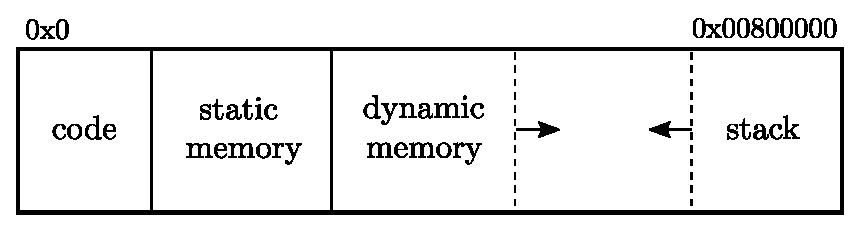
\includegraphics[scale=0.6]{memory.eps}
\caption{Memory layout}
\label{fig:memlay}
\end{figure}

\subsection*{Register allocation}
The usage of registers corresponds to the following table
\begin{table}[H]
\centering
\begin{tabular}{|l|l|}
\hline
2 & return value of function \\ \hline
8 - 24 & general registers \\ \hline
25 & auxiliary register \\ \hline
29 & stack pointer \\ \hline
30 & frame pointer \\ \hline
31 & return address \\ \hline
32 & top of dynamically allocated memory \\ \hline
\end{tabular}
\caption{Register usage}
\label{tab:regs}
\end{table}

The register 25 is used when an intermediate result needs to be temporarily stored or generally when a free register is needed for simulating a 3-address code instruction. Registers 8 - 24 hold values of variables used in the program. The allocation of the registers is controlled by 2 tables --- one mapping from variables to registers currently holding their values and second mapping registers to corresponding variables. When there is no free register to be used, the one which was allocated for the longest time is freed. The allocation holds within basic blocks --- on the transitions between blocks all registers are freed and variables are stored in memory.

%%%%
\section{Division of work}
%%%%
\begin{description}
\item [front end] Jan Wrona
\item [back end] Kateřina Žmolíková
\end{description}

%%%%
\clearpage
\appendix
%%%%
\section{Grammar rules} \label{app:grammar}
\begin{grammar}
<program> ::= <declaration_list>

<declaration_list> ::= <declaration_list> <declaration> | $\epsilon$

<declaration> ::= <function_declaration> `;' | <function_definition>

<function_declaration> ::= <type> <identifier> `(' `void' `)'
\alt <type> <identifier> `(' <parameter_type_list> `)'

<parameter_type_list> ::= <data_type> | <parameter_type_list> `,' <data_type>

<function_definition> ::= <type> <identifier> `(' `void' `)' `{' <statement_list> `}'
\alt <type> <identifier> `(' <parameter_identifier_list> `)' `{' <statement_list> `}'

<parameter_identifier_list> ::= <data_type> <identifier>
\alt <parameter_identifier_list> `,' <data_type> <identifier>

<compound_statement> ::= `{' <statement_list> `}'

<statement_list> ::= <statement_list> <statement> | $\epsilon$

<statement> ::= <variable_definition_statement> `;'
\alt <assignment_statement> `;'
\alt <selection_statement>
\alt <iteration_statement>
\alt <function_call> ';'
\alt <return_statement> ';'

<variable_definition_statement> ::= <data_type> <identifier_list>

<identifier_list> ::= <identifier> | <identifier_list> `,' <identifier>

<assignment_statement> ::= <identifier> `=' <expression>

<selection_statement> ::= `if' `(' <expression> `)' <compound_statement> `else' <compound_statement>

<iteration_statement> ::= `while' `(' <expression> `)' <compound_statement>

<function_call> ::= <identifier> `(' `)' | <identifier> `(' <expression_list> `)'

<expression_list> ::= <expression> | <expression_list> `,' <expression>

<return_statement> ::= <return> | <return> <expression>

<expression> ::= <int_lit> | <char_lit> | <string_lit>
\alt <identifier>
\alt `(' <expression> `)'
\alt `(' <data_type> ')' <expression>
\alt <function_call>
\alt `!' <expression>
\alt <expression> `*' <expression> | <expression> `/' <expression> | <expression> `\%' <expression>
\alt <expression `+' <expression> | <expression> `-' <expression>
\alt <expression> `<' <expression> | <expression> `<=' <expression>
\alt <expression> `>' <expression> | <expression> `>=' <expression>
\alt <expression> `==' <expression> | <expression> `!=' <expression>
\alt <expression> `&&' <expression> | <expression> `||' <expression>

<data_type> ::= `int' | `char' | `string'

<type> ::= `void' | <data_type>

<identifier> ::= <letter> \{ <letter> | <digit> | `_' \}

<int_lit> ::= <digit> \{ <digit> \}

<char_lit> ::= `'' <escape_char> | <char> `''

<string_lit> ::= `"' \{ <escape_char> | <char> \} `"'

<letter> ::= <lower_case_letter> | <upper_case_letter>

<lower_case_letter> ::= `a' | `b' | `c' | `d'| `e' | `f' | `g' | `h' | `i' | `j' | `k' | `l' | `m' | `n' | `o' | `p' | `q' | `r' | `s' | `t' | `u' | `v' | `w' | `x' | `y' | `z' |

<upper_case_letter> ::= `A' | `B' | `C' | `D'| `E' | `F' | `G' | `H' | `I' | `J' | `K' | `L' | `M' | `N' | `O' | `P' | `Q' | `R' | `S' | `T' | `U' | `V' | `W' | `X' | `Y' | `Z' |

<digit> ::= `0' | `1' | `2' | `3' | `4'| `5' | `6' | `7' | `8' | `9'

<char> ::= ` ' | `!' | `"' | `#' | `$' | `\%' | `&' | `(' | `)' | `*' | `+' | `,' | `-' | `.' | `/' | `:' | `;' | `<' | `=' | `>' | `?' | `@' | `[' | `\' | `]' | `^' | `_' | ``' | `{' | `|' | `}' | `~' | <digit> | <lower_case_letter> | <upper_case_letter>

<escape_char> ::= `\\' `n' | `t' | `\\' | `"' | `''
\end{grammar}

\end{document}